%!TEX root =  A_WS.tex

\section*{Practice Exam 3A}  
\markright{Practice Exam 3A}  
\addcontentsline{toc}{section}{Practice Exam 3A}

Relax.  You have done problems like these before.  Even if these problems look a bit different, just do what you can.  If you're not sure of something, please ask! You may use your calculator.  Please show all of your work and write down as many steps as you can.  Don't spend too much time on any one problem.  Do well.  And remember, ask me if you're not sure about something. \bigskip

\noindent \textbf{Over 50 points on this exam are for solving equations and inequalities. Be sure you understand what you need to show for full credit.  Using a different method will get little to no partial credit.} \bigskip

\noindent \emph{As you work, make a ``don't forget'' list of any information you need to look up or ask about.} 

\noindent \hrulefill
\bigskip


\begin{enumerate} 

\item The Sk\"arstroms want to dig a new well for water for their lake cabin.  The company charges \$900 to bring the equipment on site and draw the permit and then \$2 per foot to dig.  That means $$W=900+2F$$ where $F$ is the depth of the well (in feet) and $W$ is the cost of the well (in \$).
\begin{enumerate}
\item In their neck of the woods, wells often run 200 feet deep.  According to the equation, how much would that cost? \vfill 
\item The Sk\"arstroms have budgeted between \$1,500 and \$1,800 for the well.  Set up and solve a chain of inequalities to find the corresponding range of depths. \vfill  \vfill \vfill 
\item No such luck.  The company had to drill much deeper than hoped to find water.  The final result, wonderfully cold and clear drinking water.  And, a hefty bill for \$2,072.  How deep is their well?  Set up and solve an equation. \vfill  \vfill \vfill% 
\end{enumerate} 

\newpage

\item Ceyda starts the day by downing two cans of Red Bull, containing a total of 160 mg of caffeine.  Her body eliminates the caffeine at a rate of 12\% each hour.  That means the amount of caffeine ($C$ mg) after $H$ hours is given by the equation graphed below  $$C= 160\ast .88^H$$ 
% Su this problem appears in 5.2 #5

\begin{center}
\scalebox {.8} {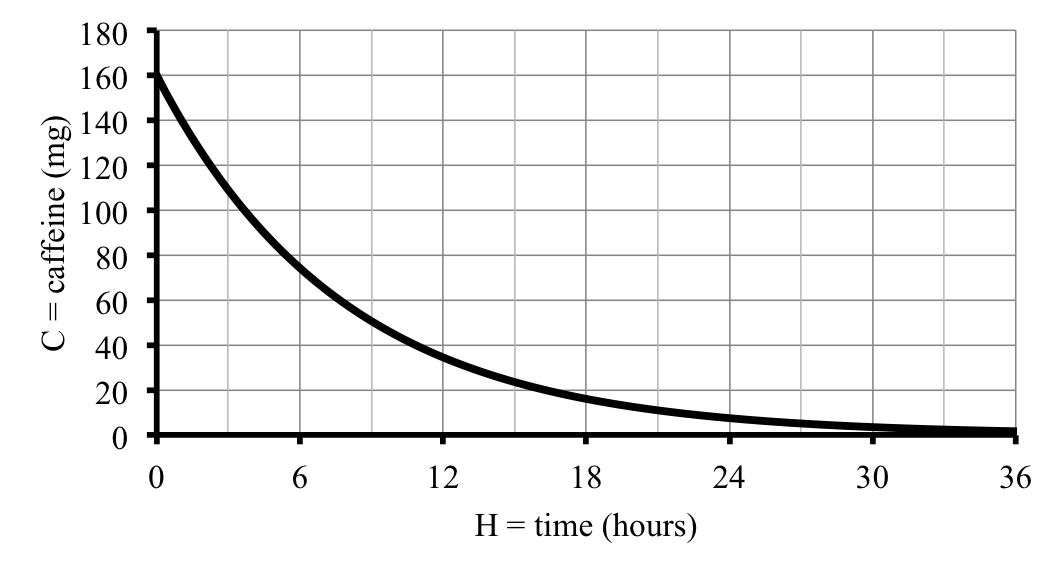
\includegraphics [width = 6in] {redbull.png}}
\end{center}

\begin{enumerate}
\item According to the equation, how much caffeine is in her body initially, after 2 hours, 5 hours, and 24 hours?  Display your answers in table.   \vfill 
\item Show show to use successive approximation to find when there will Ceyda's caffeine level first drops below 20 mg.  Answer to the nearest hour. \vfill \vfill 
\item Set up and solve an equation to determine when Ceyda's caffeine level first drops below 20 mg.  Round your answer to two decimal places. \vfill \vfill \vfill 
\end{enumerate} 

\newpage

\item Jorge deposited \$1,500 in an high yield money market account and plans to leave it there for 5 years.  The value of his account after 5 years  \$$A$ will depend on the growth factor $g$ as given by the equation $$A = 1,500g^5$$
\begin{enumerate}
\item Use the equation to complete the table. 

\begin{center}
\begin{tabular} {|c |c|c|c |c|}\hline
$g$ & ~ \quad 1.02 \quad ~& 1.03 & 1.05 &~ \quad 1.10\quad ~ \\ \hline
& & & & \\ 
$A$ & 1,656.12 & ~\hspace{1in}~&~\hspace{1in}~ & 2,415.77 \\  
\hline
\end{tabular}
\end{center}
\item Draw a graph showing how $A$ depends on the growth factor $g$. Start the $g$-axis at 1.00, instead of 0.
\begin{center}
\scalebox {.8} {
\includegraphics [width = 6in] {GraphPaper.jpg}}
\end{center}
\bigskip
\item Use your graph to estimate the growth factor if the value of Jorge's account after 5 years is \$1,780.  \vfill
\item Now set up and solve an equation to find the answer.  \vfill \vfill \vfill 
\item What is the corresponding \textbf{return on investment}?  That means calculate $r= g-1$.  The return on investment is $r$ written as a percentage. \vfill 
\end{enumerate} 

\newpage

\item A rabbit jumps so that her height above ground is given by the formula $$R = 17.6S - 22S^2$$ where $R=$ height of rabbit (feet above ground) and $S=$ time (seconds).
\begin{enumerate}
\item At what height did the rabbit start her jump? \vfill 
\item Can the rabbit jump over a 3 foot fence?  Calculate the exact maximum height of the rabbit to decide. \vfill \vfill 
\item How long does it take the rabbit to get 2 feet in the air and when is she at that height again? Set up and solve the appropriate equation to find the answers.  \vfill \vfill \vfill \vfill \vfill
\end{enumerate} 

%%% END

\end{enumerate}



